%% Progetto di linguaggi di programmazione - Gianluca Grilletti e Giovanni Barbarino
%% Semantica Fully Abstract per PCF


\documentclass{beamer}

\usepackage[utf8]{inputenc}
\usepackage{default}
\usepackage{amssymb}
\usepackage{stmaryrd}
\usepackage{graphicx}
\usepackage{caption}
\usepackage{subcaption}
\usepackage{tikz}
\usetikzlibrary{arrows,automata}

\newcommand{\eqobs}{\stackrel{\text{obs}}{=}}
\newcommand{\limp}{\mathbin{{-}\mkern-3.5mu{\circ}}}
\newcommand{\tnode}[4]{\node (#1_u) at (#2,#3+0.1) [minimum size=2pt, opacity=0] 		       {#4};
		       \node (#1_d) at (#2,#3-0.1) [minimum size=2pt, opacity=0] {#4};
		       \node (#1) at (#2,#3) [minimum size=2pt] {#4};}


% immagini
\graphicspath{{immagini/}}




\usetheme{Darmstadt}

\title{Un modello fully abstract del PCF}
% \subtitle{Vuoi fare un gioco con me?}
\author{Grilletti Gianluca \and Barbarino Giovanni}
\institute[Unipi]{Università di Pisa}


\begin{document}

\small


\section{Il linguaggio PCF}
\subsection{La sintassi}

%titolo
\begin{frame}
	%\frametitle{Il linguaggio PCF}
	\maketitle
	
\end{frame}



% tavolo e carte
\begin{frame}
	
	Come rappresentiamo i giochi (il tavolo insomma)
	
	\begin{tikzpicture}
	 \node (inv) at (0,0) [minimum size=2pt] {};
	 \draw [fill=blue, opacity=.5] (7,-5) rectangle (3,-1);
	 \node (A) at (5,-3) [minimum size=2pt, scale=4] {A};
	 \node (P) at (3.5,-4.5) [minimum size=2pt, scale=2.5] {P};
	 \node (O) at (3.5,-1.5) [minimum size=2pt, scale=2.5] {O};
	 
	 \node (st_1) at (6,-5.5) [minimum size=2pt, scale=1.5] {$*_1$};
	 \only<2-> {\node (st_2) at (6,-0.5) [minimum size=2pt, scale=1.5] {$*_2$};}
	 \only<3->{\node (ri_1) at (4.5,-5.5) [minimum size=2pt, scale=1.5] {$n_1$};}
	 \only<4->{\node (ri_2) at (4.5,-0.5) [minimum size=2pt, scale=1.5] {$n_2$};}
	 
	  \only<2->{\draw[->] [out=80,in=280] (st_1) to (st_2);}
	  \only<3->{\draw[->] [out=250,in=30] (st_2) to (ri_1);}
	  \only<4->{\draw[->] [out=80,in=280] (ri_1) to (ri_2);}
	\end{tikzpicture}

	
	
	
\end{frame}






\end{document}
